% arara: lualatex: { synctex: on, shell: off }
% arara: biber
% arara: lualatex: { synctex: on, shell: off }
% arara: sumatrapdf
\documentclass[../main.tex]{subfiles}

\begin{document}
The figures in this appendix are included in the following work and are reproduced with permission:

\begin{itemize}
\item[] Burke, S., Burke, U., Mathieu, O., Osorio, I., Keesee, C.,
Morones, A., Petersen, E. L., Wang, W., DeVerter, T.,
Oehlschlaeger, M. A., Rhodes, B., Hanson, R. K., Davidson, D. F.,
Weber, B. W., Sung, C.-J., Santner, J., Ju, Y., Haas, F. M.,
Dryer, F. L., Volkov, E., Nilsson, E., Konnov, A., Alrefae, M.,
Khaled, F., Farooq, A., Dirrenberger, P., Glaude, P.-A., and
Battin-Leclerc, F. ``An Experimental and Modeling Study of
Propene Oxidation. Part 2: Ignition Delay Time and Flame Speed
Measurements.'' \textit{Combust. Flame}, (Submitted).
\end{itemize}

Propene is a foundational fuel that is an important step in the hierarchy
of chemical kinetic models. Despite this, very few experiments have
been conducted for propene at high-pressure, and low-to-intermediate
temperature conditions. The data presented here substantially expand
the available data sets for model validation.

In addition, this study was conducted in concert with collaborators at
the National University of Ireland (NUI) at Galway, Texas A\&M
University, the King Abdullah University of Science and Technology,
Stanford University, and Rensselaer Polytechnic Institute. The facilities
utilized included two different RCMs and six different shock tubes; as such,
this study represents one of the first comprehensive comparisons of
homogeneous ignition in many experimental facilities.

That such a comparison is warranted is shown by
\cref{fig:pressure-trace-comp,fig:ign-delay-comp}. \Cref{fig:pressure-trace-comp}
shows a comparison of the pressure traces from an experiment in the RCMs
at UConn and NUI Galway. It is clear that, although the EOC pressures are
similar, the pressure profiles pre- and post-EOC are quite difference. The
outcome of this difference in profile is evident in the difference in ignition
delay displayed in \cref{fig:ign-delay-comp}. The ignition delays measured
in the UConn RCM are shorter than those measured in the NUI Galway RCM
in part because the pressure loss---and hence temperature loss---in the
UConn RCM is less.

\begin{figure}
    \begin{floatrow}
        \ffigbox
            {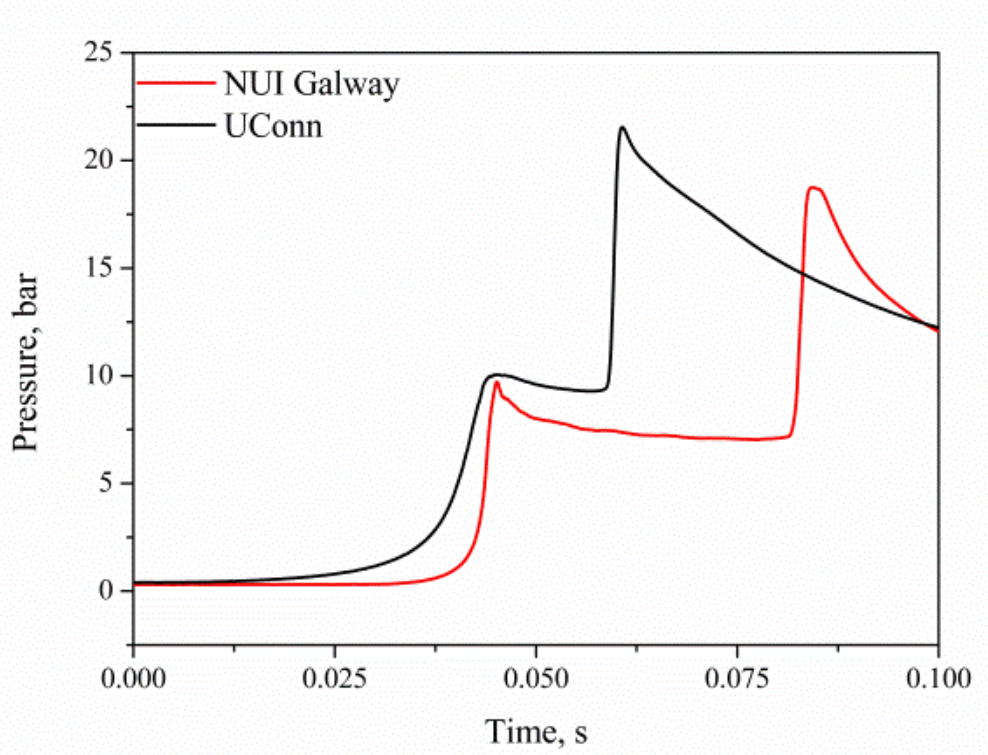
\includegraphics[width=7.9cm]{E-Propene/pressure-trace-comp}}
            {\caption{Comparison of pressure traces between the UConn and
            NUI Galway RCMs. $P_C=\SI{10}{\atmosphere}$, $T_C\approx\SI{1040}{\kelvin}$,
            $\phi=1.0$, \SI{12}{\percent} \ce{O2}.}
            \label{fig:pressure-trace-comp}}
        \ffigbox
            {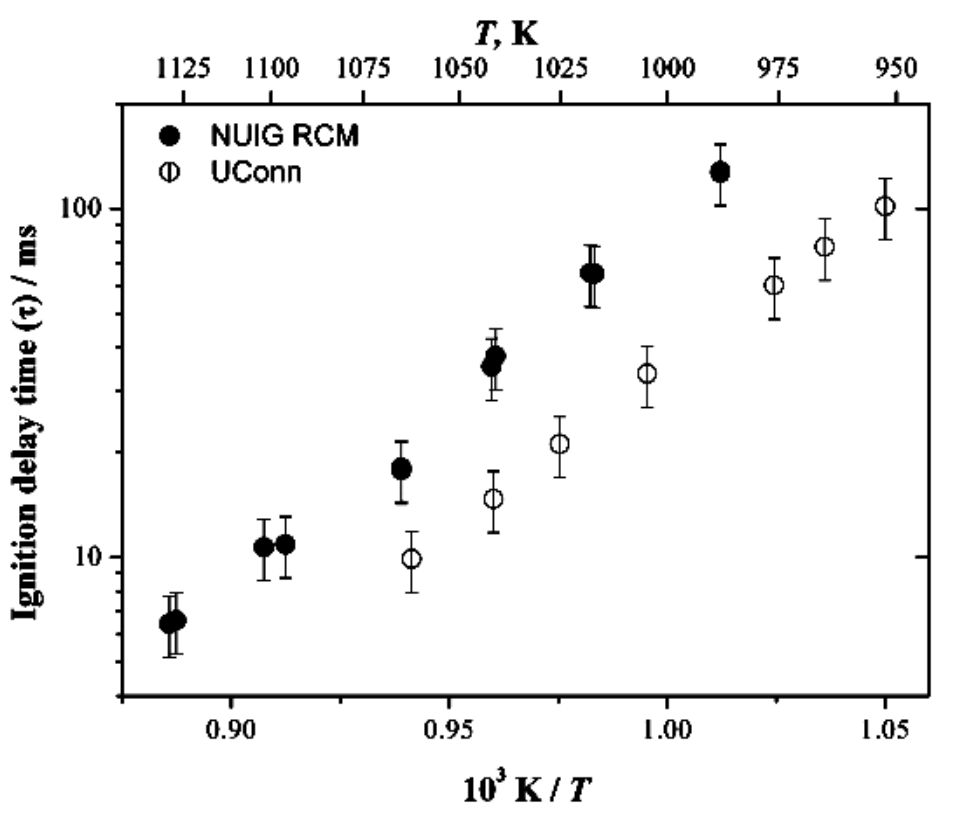
\includegraphics[width=7.9cm]{E-Propene/ign-delay-comp}}
            {\caption{Comparison of ignition delays of propene measured
            in the UConn and NUI Galway RCMs. $P_C=\SI{10}{\atmosphere}$,
            $\phi=1.0$, \SI{12}{\percent} \ce{O2}.}
            \label{fig:ign-delay-comp}}
    \end{floatrow}
\end{figure}

\Crefrange{fig:phi-10-air}{fig:40-atm-4o2} compare the results of the experiments in the
various facilities to each other and to a model for propene developed
in the work cited above. The symbols represent experimental data; simulations
of the NUI Galway RCM and shock tube experiments are represented by solid lines;
and simulations of the UConn RCM experiments are represented by dashed lines.
In general, the agreement among the experiments and between the experiments
and the model is quite good. Most importantly, the experiments are well
modeled by the kinetic mechanism when the proper facility effects are
applied to the simulation.

\begin{figure}
    \begin{floatrow}
        \ffigbox
            {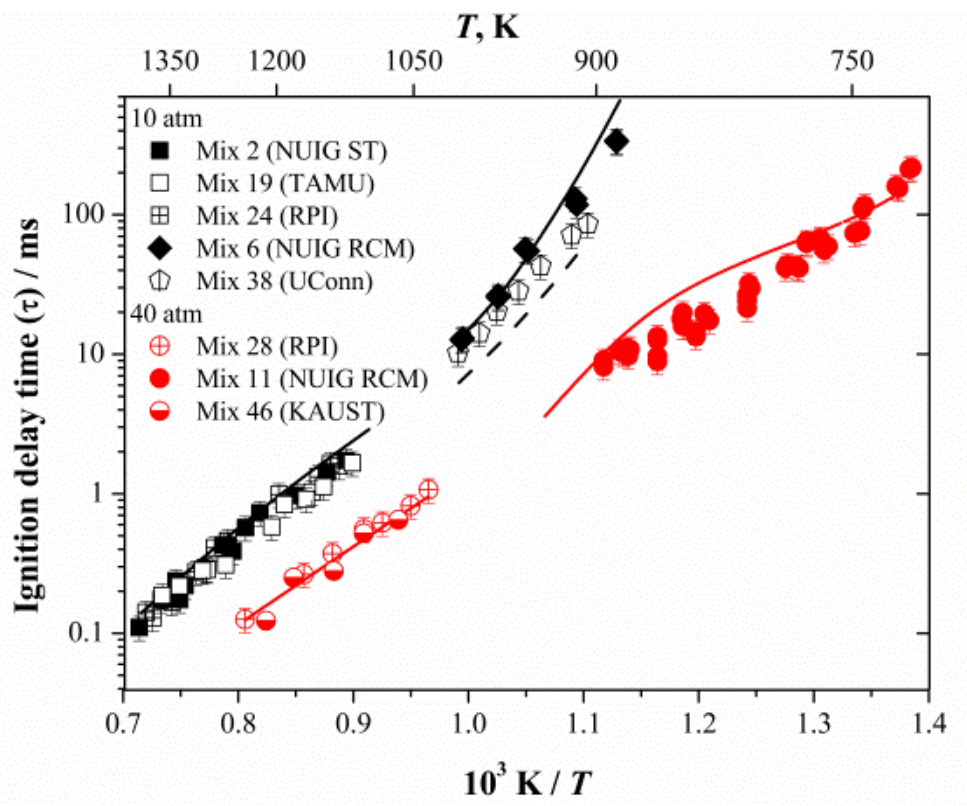
\includegraphics[width=7.9cm]{E-Propene/phi-10-air}}
            {\caption[Ignition delays of propene in stoichiometric
            mixture with air at\newline two pressures]{Ignition delays of propene in stoichiometric
            mixture with air at two pressures}
            \label{fig:phi-10-air}}
        \ffigbox
            {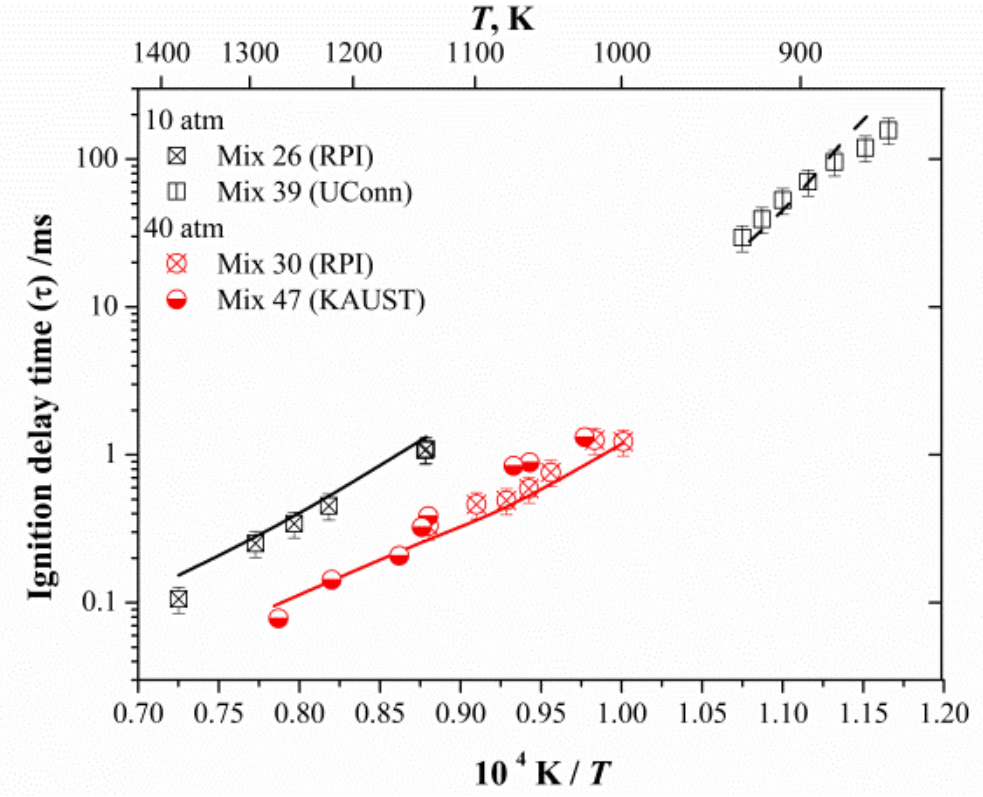
\includegraphics[width=7.9cm]{E-Propene/phi-20-air}}
            {\caption{Ignition delays of propene in $\phi=2.0$
            mixture with air at two pressures}
            \label{fig:phi-20-air}}
    \end{floatrow}
\end{figure}

\begin{figure}
    \begin{floatrow}
        \ffigbox
            {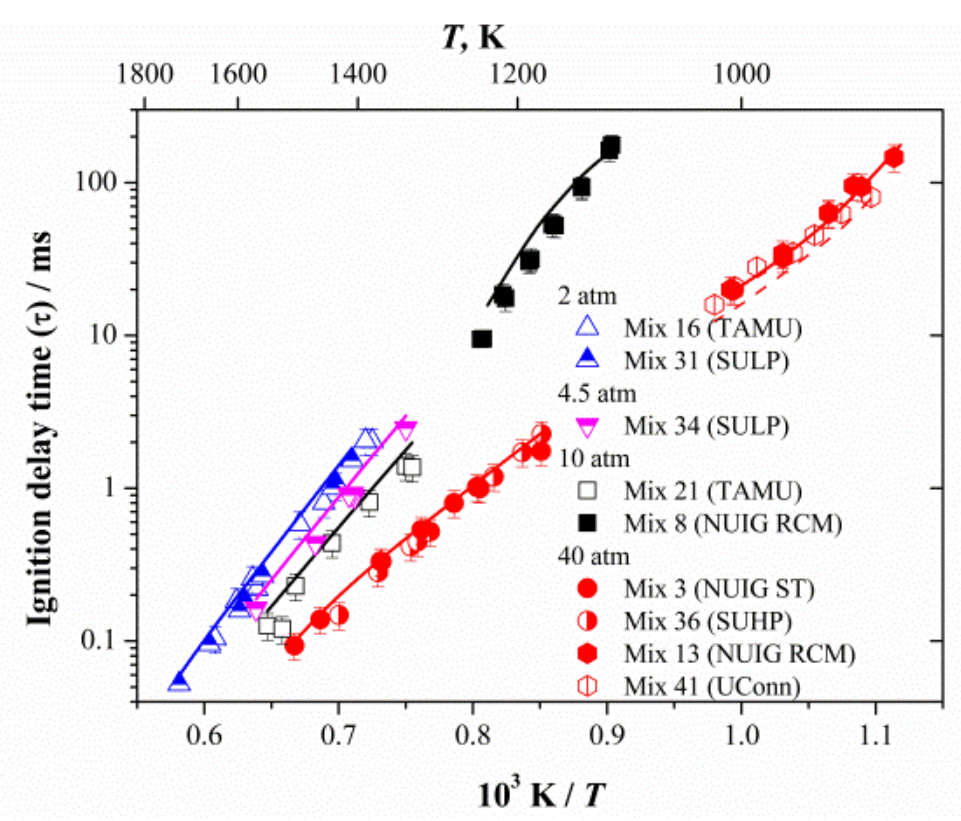
\includegraphics[width=7.9cm]{E-Propene/phi-10-4o2}}
            {\caption{Ignition delays of propene with \SI{4}{\percent}
            \ce{O2}, $\phi=1.0$}
            \label{fig:phi-10-4o2}}
        \ffigbox
            {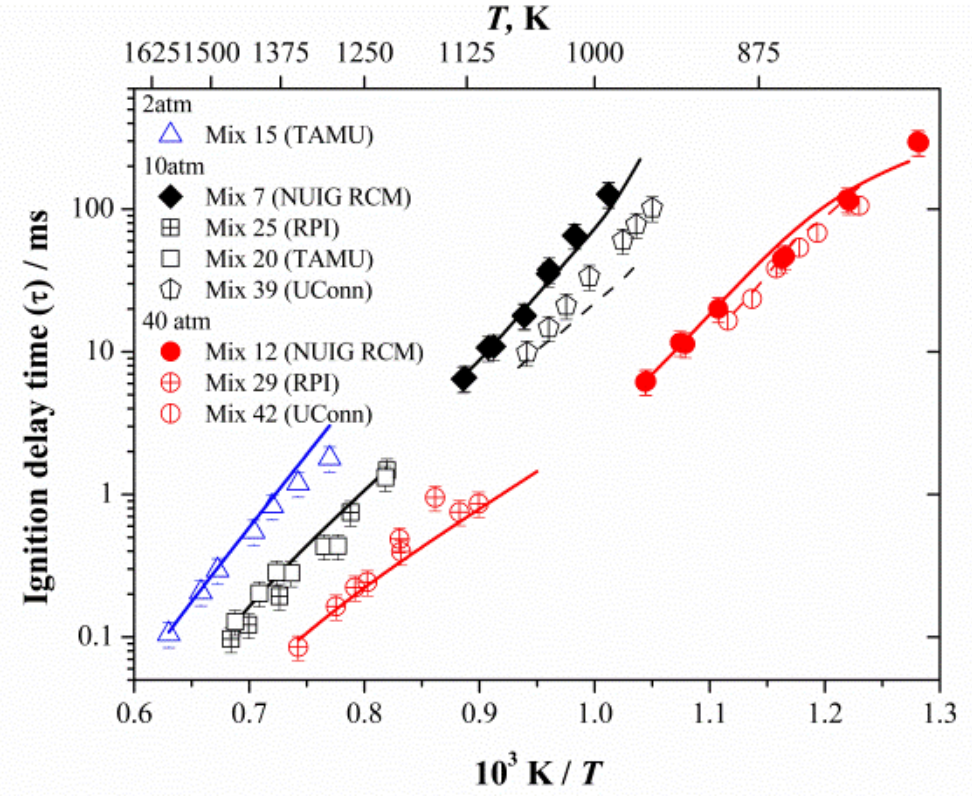
\includegraphics[width=7.9cm]{E-Propene/phi-10-12o2}}
            {\caption{Ignition delays of propene with \SI{12}{\percent}
            \ce{O2}, $\phi=1.0$}
            \label{fig:phi-10-12o2}}
    \end{floatrow}
\end{figure}

\begin{figure}
    \begin{floatrow}
        \ffigbox
            {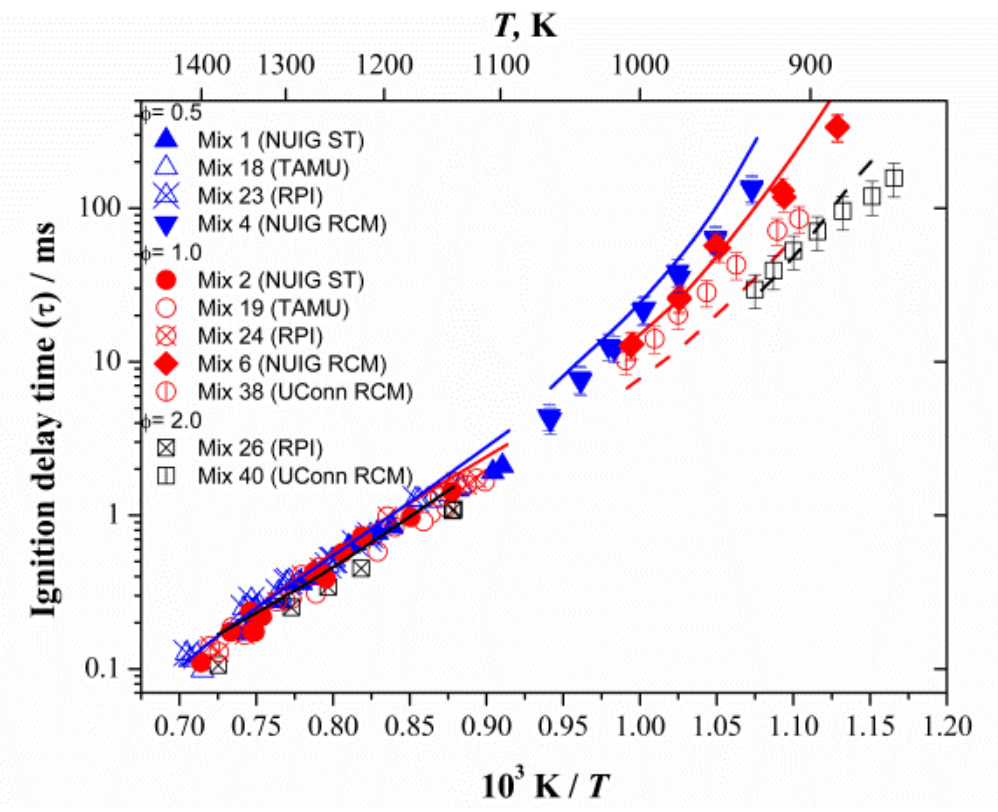
\includegraphics[width=7.9cm]{E-Propene/10-atm-air}}
            {\caption{Ignition delays of propene with mixtures of air at
            \SI{10}{\atmosphere} for three equivalence ratios}
            \label{fig:10-atm-air}}
    \end{floatrow}
\end{figure}

\begin{figure}
    \begin{floatrow}
        \ffigbox
            {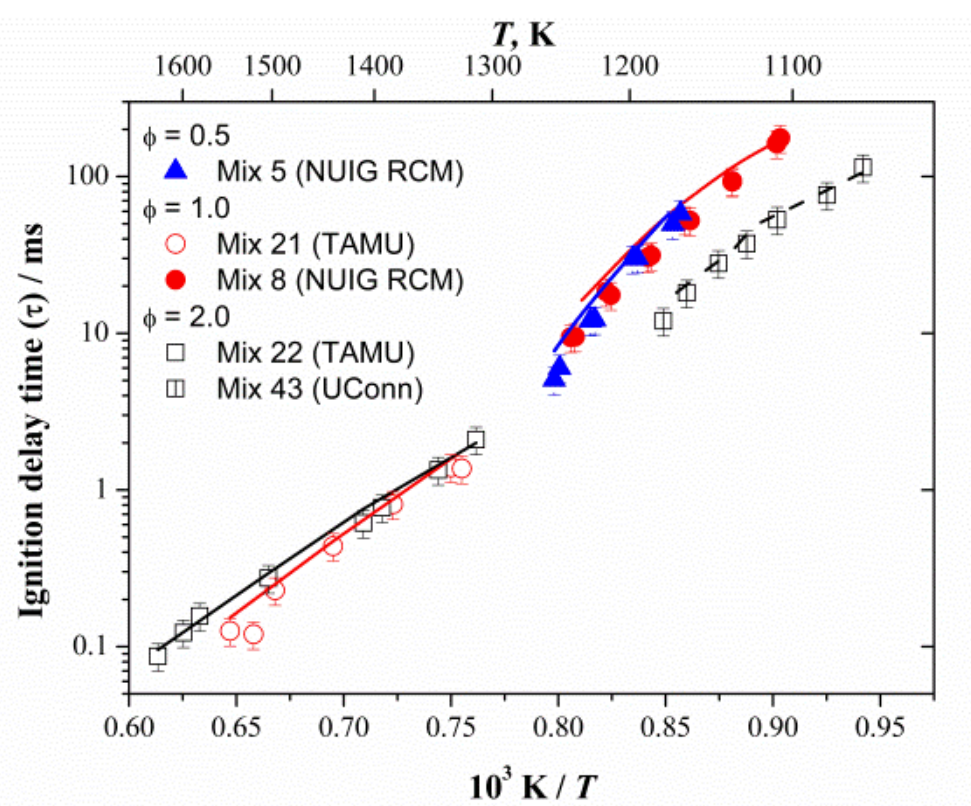
\includegraphics[width=7.9cm]{E-Propene/10-atm-4o2}}
            {\caption[Ignition delays of propene with \SI{4}{\percent}
            \ce{O2} at \SI{10}{\atmosphere} for three\newline equivalence ratios]{Ignition delays of propene with \SI{4}{\percent}
            \ce{O2} at \SI{10}{\atmosphere} for three equivalence ratios}
            \label{fig:10-atm-4o2}}
        \ffigbox
            {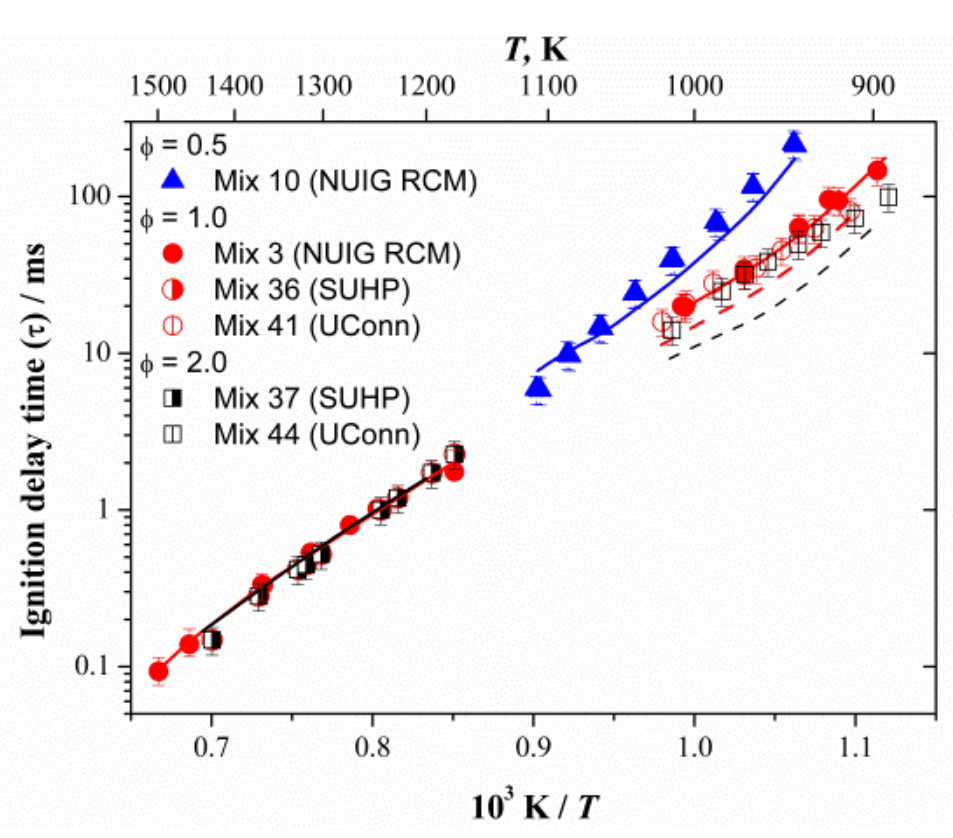
\includegraphics[width=7.9cm]{E-Propene/40-atm-4o2}}
            {\caption[Ignition delays of propene with \SI{4}{\percent}
            \ce{O2} at \SI{40}{\atmosphere} for three\newline equivalence ratios]{Ignition delays of propene with \SI{4}{\percent}
            \ce{O2} at \SI{40}{\atmosphere} for three equivalence ratios}
            \label{fig:40-atm-4o2}}
    \end{floatrow}
\end{figure}

\end{document}
